\documentclass[11pt, 
               %hyperref={colorlinks},
               aspectratio=169]{beamer}
\usetheme{Singapore}

\usepackage[utf8]{inputenc}
\usepackage[T1]{fontenc}
\usepackage[american]{babel} % artficact from theme
\usepackage{graphicx}

\usepackage[natbib=true,style=authoryear,backend=bibtex,useprefix=true]{biblatex}
\setbeamercolor*{bibliography entry title}{fg=black}
\setbeamercolor*{bibliography entry location}{fg=black}
\setbeamercolor*{bibliography entry note}{fg=black}
\setbeamertemplate{bibliography item}{}
\setbeamerfont{caption}{size=\footnotesize}
\renewcommand*{\bibfont}{\scriptsize}
\addbibresource{bibliography.bib}

\author{Patrick Hall}
\title{Machine Learning Interpretability}
\subtitle{The Good, the Bad, and the Ugly}
\logo{
\includegraphics[height=8pt]{img/h2o_logo.png}}
\institute{H\textsubscript{2}O.ai}
\date{Aug. 1 2018}
\subject{Machine Learning Interpretability Guidance for Practitioners}

\begin{document}
	
	\maketitle
	
	\begin{frame}
		\frametitle{Contents}
		\tableofcontents{}
	\end{frame}

%-------------------------------------------------------------------------------
	\section{Front Matter}
%-------------------------------------------------------------------------------
	
	\begin{frame}
	
		\frametitle{Obligatory Front Matter}
		
			\begin{itemize}
				
				\item \textbf{What is interpretation?} “The	ability	to explain or to present in understandable terms to	a human.” \cite{been_kim1}
				
				\item \textbf{What is a good interpretation?} "When you can no longer keep asking why." \cite{gilpin2018explaining}
				
				\item \textbf{Why should you care?}
				\begin{itemize}
					\item Addressing accidental or intentional discrimination.
					\item Preventing malicious hacking and adversarial attacks.
					\item Enabling regulatory compliance and increased financial margins.
				\end{itemize}
				
			\end{itemize}
		
		
	\end{frame}

% Defintion
% Good explanation is when I stop asking why
% Donoho quote

%-------------------------------------------------------------------------------
	\subsection{Notation}
%-------------------------------------------------------------------------------
	
	\begin{frame}
	
		\frametitle{Notation}
		
			\begin{itemize}
			\item \textbf{Spaces}.  
			\begin{itemize}
				\item The input features come from a set  $\mathcal{X}$ contained in a \textit{P}-dimensional input space (i.e. $\mathcal{X} \subset \mathbb{R}^P)$.  
				\item The output responses come from a set $\mathcal{Y}$ contained in a $C$-dimensional output space (i.e. $\mathcal{Y} \subset \mathbb{R}^C$).
			\end{itemize}	
			\bigskip	
			\item \textbf{Dataset}. A dataset $\mathbf{D}$ consists of $N$ tuples of observations:\\ $[(\mathbf{x}^{(0)},\mathbf{y}^{(0)}), (\mathbf{x}^{(1)},\mathbf{y}^{(1)}), \dots, (\mathbf{x}^{(N-1)},\mathbf{y}^{(N-1)})], \mathbf{x}^{(i)} \in \mathcal{X}, \mathbf{y}^{(i)} \in \mathcal{Y}$.\\
			\begin{itemize}
				\item The input data $\mathbf{X}$ is composed of the set of row vectors $\mathbf{x}^{(i)}$. 
				\begin{itemize}
					\item let $\mathcal{P}$ be the set of features  $\{X_0, X_1, \dots, X_{P-1}\}$, where $X_j = \left[x_{j}^{(0)}, x_{j}^{(1)}, \dots, x_{j}^{(N-1)} \right]^T$.
					\item then each $i$-th observation denoted as $\mathbf{x}^{(i)} = \left[x_0^{(i)}, x_1^{(i)}, \dots, x_{P-1}^{(i)} \right]$ is an instance of $\mathcal{P}$.
				\end{itemize}
			\end{itemize}
		\end{itemize}
	
	\end{frame}

%-------------------------------------------------------------------------------
    \subsection{Learning Problem}
%-------------------------------------------------------------------------------
	
	\begin{frame}
	
		\frametitle{Proposed Updates to the Learning Problem}
		
		\begin{figure}[htb]
			\begin{center}
				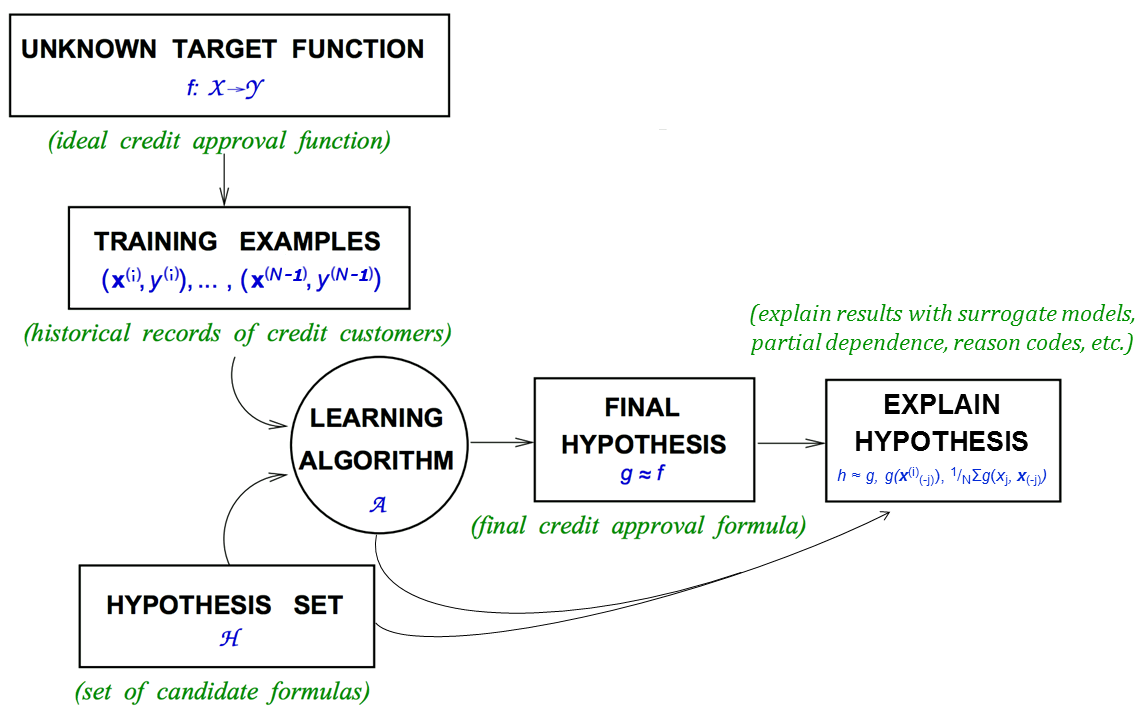
\includegraphics[height=125pt]{img/learning_problem.png}
				\label{fig:learning_problem}
			\end{center}
		\end{figure}
		
		The learning problem. Adapted from \textit{Learning From Data}, \cite{lfd}.
		
	\end{frame}

%-------------------------------------------------------------------------------
	\section{Surrogate DT}
%-------------------------------------------------------------------------------

	\begin{frame}
	
		\frametitle{Surrogate Decision Trees}
		
		\vspace{-10 pt}
		
		\begin{figure}[htb]
			\begin{center}
				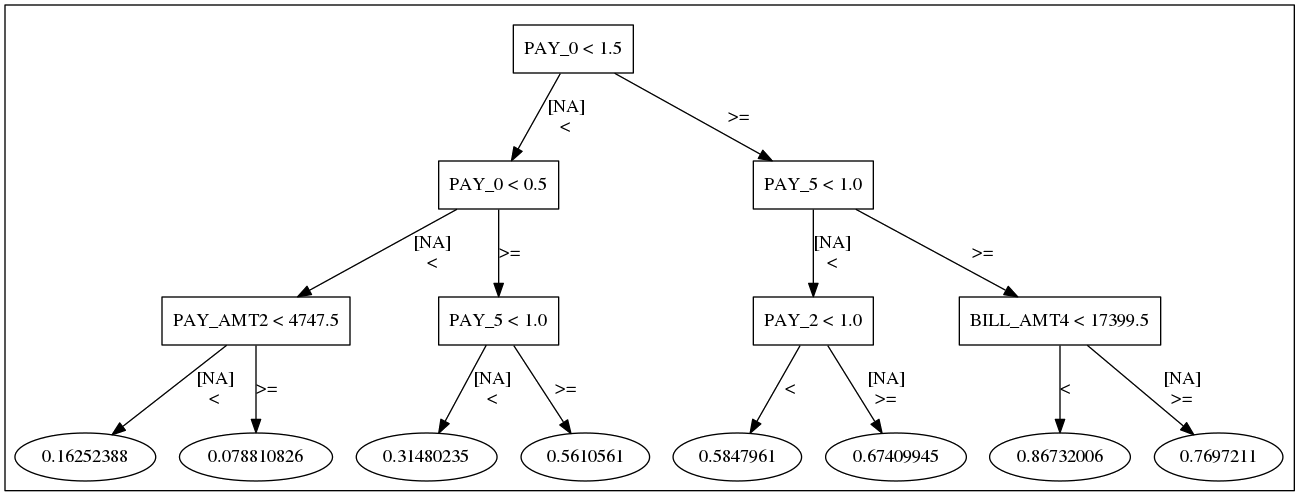
\includegraphics[height=100pt]{img/dt_surrogate.png}
				\label{fig:dt_surrogate}
			\end{center}
		\end{figure}
		
		\vspace{-10 pt}
		
		\begin{itemize}
			
			\item Given a learned function $g$ and set of predictions, $g(\mathbf{X}) = \hat{\mathbf{Y}}$, a surrogate decision tree model can be trained: $ \mathbf{X},\hat{\mathbf{Y}} \xrightarrow{\mathcal{A}_{\text{surrogate}}} h_{\text{tree}}$.
	
			\item $h_{\text{tree}}$ displays a low-fidelity flow chart of $g$'s decision making process, important features in $g$, and important interactions in $g$.	
		
		\end{itemize}
		
	\end{frame}
	
	\begin{frame}
	
		\frametitle{Surrogate Decision Trees}
		
		\vspace{-10 pt}
		
		\begin{itemize}
			
			\item Always use error measures to assess the trustworthiness of $h_{\text{tree}}$.

			\item Prescribed methods (\cite{dt_surrogate1}; \cite{dt_surrogate2}) for training $h_{\text{tree}}$ do exist. In practice, straightforward cross-validation approaches are typically sufficient. 
			
			\item Comparing cross-validated error to standard training error can give an indication of the stability of the single tree model, $h_{\text{tree}}$.
			
			\item \cite{lime-sup} use local linear surrogate models, $h_{\text{glm}}$, in $h_{\text{tree}}$ leaf nodes to increase overall surrogate model accuracy while retaining a high degree of interpretability.

			\item $h_{\text{tree}}$ can provide low-fidelity explanations for model mechanisms in the original feature space if $g$ is defined to include feature extraction.
			
		\end{itemize}
		
	\end{frame}

% Use CV error
% Map between original features and predictions

%-------------------------------------------------------------------------------
	\section{Partial Dependence}
%-------------------------------------------------------------------------------

	\begin{frame}
		\frametitle{Partial Dependence - \textit{Description}}
	\end{frame}

	\begin{frame}
		\frametitle{Partial Dependence - \textit{Recommendations}}
	\end{frame}

%-------------------------------------------------------------------------------
	\section{ICE}
%-------------------------------------------------------------------------------

	\begin{frame}
		\frametitle{Individual Conditional Expectation (ICE) - \textit{Description}}
	\end{frame}

	\begin{frame}
		\frametitle{Individual Conditional Expectation (ICE) - \textit{Recommendations}}
	\end{frame}

%-------------------------------------------------------------------------------
	\section{LIME}
%-------------------------------------------------------------------------------

	\begin{frame}
		\frametitle{Local Interpretable Model-agnostic Explanations (LIME) - \textit{Description}}
	\end{frame}

	\begin{frame}
		\frametitle{Local Interpretable Model-agnostic Explanations (LIME) - \textit{Recommendations}}
	\end{frame}

% Map between original features and predictions
% Low Fidelity, Sparse, i.e. human readable
% Unstructured data
% Variants: K-LIME, LIME-SUP

%-------------------------------------------------------------------------------
	\section{Tree Shap}
%-------------------------------------------------------------------------------

	\begin{frame}
		\frametitle{Tree Shap - \textit{Description}}
	\end{frame}

	\begin{frame}
		\frametitle{Tree Shap - \textit{Recommendations}}
	\end{frame}

% High fidelity

%-------------------------------------------------------------------------------
	\section{Recommendations}
%-------------------------------------------------------------------------------

	\begin{frame}
		\frametitle{Closing Recommendations}
	\end{frame}

% generative methods can be less useful b/c people want to see explanations on there on data 
% Show High Fidelity and Low Fidelity
% Testing

%-------------------------------------------------------------------------------
%	References
%-------------------------------------------------------------------------------


	\begin{frame}
		\frametitle{References}
		\printbibliography
	\end{frame}

\end{document}